\documentclass[../main.tex]{subfiles}
\begin{document}
	
	The finite element method is a powerful tool for solving differential equations.
	The method can easily deal with complex geometries and higher-order approximations of the solution. Figure \ref{fig:img_1} shows a two-dimensional domain with a non-trivial
	geometry. The idea is to divide the domain into triangles (elements) and seek
	a polynomial approximations to the unknown functions on each triangle. The
	method glues these piecewise approximations together to find a global solution.
	Linear and quadratic polynomials over the triangles are particularly popular.
	
	\begin{figure}[H]
		\centering
		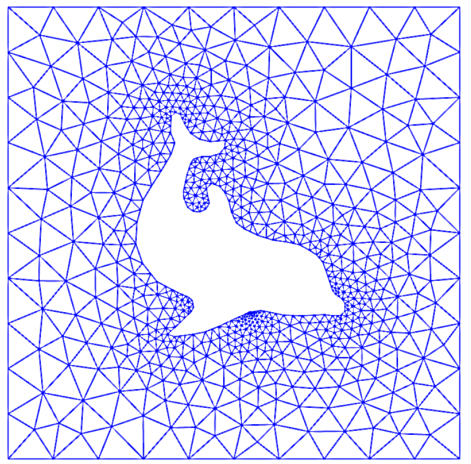
\includegraphics[width=0.7\linewidth]{img_1}
		\caption{Domain for flow around a dolphin.}
		\label{fig:img_1}
	\end{figure}
	
	Many successful numerical methods for differential equations, including the finite element method, aim at approximating the unknown function by a sum
	\begin{equation}\label{eqa1}
		u(x)=\sum_{i=0}^{N} c_{i} \psi_{i}(x),
	\end{equation}
	where $\psi_{i}(x)$ are prescribed functions and $c_{0}, \ldots, c_{N}$ are unknown coefficients to be determined. Solution methods for differential equations utilizing (\ref{eqa1}) must have a \textit{principle} for constructing $N+1$ equations to determine $c_{0}, \ldots, c_{N}$. Then there is a \textit{machinery} regarding the actual constructions of the equations for $c_{0}, \ldots, c_{N}$, in a particular problem. Finally, there is a solve phase for computing the solution $c_{0}, \ldots, c_{N}$ of the $N+1$ equations.
	
	Especially in the finite element method, the machinery for constructing the discrete equations to be implemented on a computer is quite comprehensive, with many mathematical and implementational details entering the scene at the same time. From an ease-of-learning perspective it can therefore be wise to introduce the computational machinery for a trivial equation: $u=f$. Solving this equation with $f$ given and $u$ on the form (\ref{eqa1}) means that we seek an approximation $u$ to $f$. This approximation problem has the advantage of introducing most of the finite element toolbox, but with postponing demanding topics related to differential equations (e.g., integration by parts, boundary conditions, and coordinate mappings). This is the reason why we shall first become familiar with finite element \textit{approximation} before addressing finite element methods for differential equations.
	
	First, we refresh some linear algebra concepts about approximating vectors in vector spaces. Second, we extend these concepts to approximating functions in function spaces, using the same principles and the same notation. We present examples on approximating functions by global basis functions with support throughout the entire domain. Third, we introduce the finite element type of local basis functions and explain the computational algorithms for working with such functions. Three types of approximation principles are covered: 1) the least squares method, 2) the $L_{2}$ projection or Galerkin method, and 3 ) interpolation or collocation.
	%\setcounter{chapter}{1}
\chapter{ Approximation of vectors}
	\label{chap:chap_1}
	\pagenumbering{arabic}
	\setcounter{page}{1}
	\noindent We shall start with introducing two fundamental methods for determining the
	coefficients $c_{i}$
	in (\ref{eqa1}) and illustrate the methods on approximation of vectors,
	because vectors in vector spaces give a more intuitive understanding than starting
	directly with approximation of functions in function spaces. The extension
	from vectors to functions will be trivial as soon as the fundamental ideas are
	understood.
	
	The first method of approximation is called the \textit{least squares} method and
	consists in finding $c_{i}$ such that the difference \textit{u} - \textit{f}, measured in some norm, is
	minimized. That is, we aim at finding the best approximation \textit{u} to \textit{f} (in some
	norm). The second method is not as intuitive: we find u such that the error
	\textit{u} - \textit{f} is orthogonal to the space where we seek \textit{u}. This is known as \textit{projection},
	or we may also call it a \textit{Galerkin method}. When approximating vectors and
	functions, the two methods are equivalent, but this is no longer the case when
	applying the principles to differential equations
	
	\section[Approximation of planar vectors]{Approximation of planar vectors}
	\label{sec:sec_1_1}
	\noindent Suppose we have given a vector \textit{\textbf{f}} = (3, 5) in the \textit{xy} plane and that we want to
	approximate this vector by a vector aligned in the direction of the vector \textit{(a, b)}.
	Figure \ref{fig:img_2} depicts the situation.
	
	We introduce the vector space \textit{V} spanned by the vector $\psi_{0}$ = (a, b):
	
	\begin{figure}[H]
		\centering
		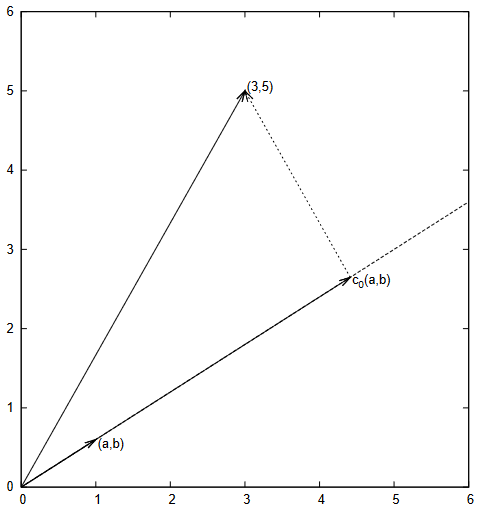
\includegraphics[width=0.7\linewidth]{img_2}
		\caption{Approximation of a two-dimensional vector by a one-dimensional vector.}
		\label{fig:img_2}
	\end{figure}
	\begin{equation}\label{eqa2}
		V=\operatorname{span}\left\{\psi_{0}\right\}
	\end{equation}
	
	\noindent We say that $\psi_{0}$ is a basis vector in the space $V$. Our aim is to find the vector $\boldsymbol{u}=c_{0} \psi_{0} \in V$ which best approximates the given vector $\boldsymbol{f}=(3,5)$. A reasonable criterion for a best approximation could be to minimize the length of the difference between the approximate u and the given $\boldsymbol{f}$. The difference, or error $e=\boldsymbol{f}-\boldsymbol{u}$, has its length given by the \textit{norm}
	$$
	\|e\|=(e, e)^{\frac{1}{2}},
	$$
	where $(e, e)$ is the \textit{inner product} of $e$ and itself. The inner product, also called \textit{scalar product} or \textit{dot product}, of two vectors $\boldsymbol{u}=\left(u_{0}, u_{1}\right)$ and $\boldsymbol{v}=\left(v_{0}, v_{1}\right)$ is defined as
	\begin{equation}\label{eqa3}
		(\boldsymbol{u}, \boldsymbol{v})=u_{0} v_{0}+u_{1} v_{1}.
	\end{equation}
	
	\noindent \textbf{Remark 1.} We should point out that we use the notation $(\cdot, \cdot)$ for two different things: $(a, b)$ for scalar quantities $a$ and $b$ means the vector starting in the origin and ending in the point $(a, b)$, while $(\boldsymbol{u}, \boldsymbol{v})$ with vectors $\boldsymbol{u}$ and $\boldsymbol{v}$ means the inner product of these vectors. Since vectors are here written in boldface font there should be no confusion. We may add that the norm associated with this inner product is the usual Eucledian length of a vector.
	\bigbreak
	\noindent \textbf{Remark 2.} It might be wise to refresh some basic linear algebra by consulting a textbook. Exercises \hyperref[sec:sec_10_1]{1} and \hyperref[sec:sec_10_1]{2} suggest specific tasks to regain familiarity with fundamental operations on inner product vector spaces.
	\bigbreak
	\noindent \textbf{The least squares method}. We now want to find $c_{0}$ such that it minimizes $\|e\|$. The algebra is simplified if we minimize the square of the norm, $\|e\|^{2}=$ $(e, e)$, instead of the norm itself. Define the function
	\begin{equation}\label{eqa4}
		E\left(c_{0}\right)=(e, e)=\left(\boldsymbol{f}-c_{0} \psi_{0}, \boldsymbol{f}-c_{0} \psi_{0}\right).
	\end{equation}
	We can rewrite the expressions of the right-hand side in a more convenient form for further work:
	\begin{equation}
		\label{eqa5}
		E\left(c_{0}\right)=(\boldsymbol{f}, \boldsymbol{f})-2 c_{0}\left(\boldsymbol{f}, \psi_{0}\right)+c_{0}^{2}\left(\psi_{0}, \psi_{0}\right).
	\end{equation}
	The rewrite results from using the following fundamental rules for inner product spaces:
	
	\begin{equation}\label{eqa6}
		(\alpha u, v)=\alpha(u, v), \quad \alpha \in \mathbb{R},
	\end{equation}
	\begin{equation}\label{eqa7}
		(u + v, w)=(u, w)+(v, w),
	\end{equation}
	\begin{equation}\label{eqa8}
		(u, v)= (v, u)
	\end{equation}
	\indent Minimizing $E\left(c_{0}\right)$ implies finding $c_{0}$ such that
	$$
	\frac{\partial E}{\partial c_{0}}=0.
	$$
	Differentiating (\ref{eqa5}) with respect to $c_{0}$ gives
	\begin{equation}\label{eqa9}
		\frac{\partial E}{\partial c_{0}}=-2\left(\boldsymbol{f}, \psi_{0}\right)+2 c_{0}\left(\psi_{0}, \psi_{0}\right)
	\end{equation}
	Setting the above expression equal to zero and solving for $c_{0}$ gives
	\begin{equation}\label{eqa10}
		c_{0}=\frac{\left(\boldsymbol{f}, \psi_{0}\right)}{\left(\psi_{0}, \psi_{0}\right)}
	\end{equation}
	which in the present case with $\psi_{0}=(a, b)$ results in
	\begin{equation}\label{eqa11}
		c_{0}=\frac{3 a+5 b}{a^{2}+b^{2}}.
	\end{equation}
	For later, it is worth mentioning that setting the key equation (\hyperref[eqa9]{9}) to zero can be rewritten as
	$$
	\left(f-c 0 \psi_{0}, \psi_{0}\right)=0,
	$$
	or
	\begin{equation}\label{eqa12}
		\left(e, \psi_{0}\right)=0.
	\end{equation}
	\textbf{The projection method.} We shall now show that minimizing $\|e\|^{2}$ implies that $\boldsymbol{e}$ is orthogonal to \textit{any} vector $\boldsymbol{v}$ in the space $V$. This result is visually quite clear from Figure \hyperref[fig:img_2]{2} (think of other vectors along the line $(a, b)$ : all of them will lead to a larger distance between the approximation and $\boldsymbol{f})$. To see this result mathematically, we express any $v \in V$ as $v=s \psi_{0}$ for any scalar parameter $s$, recall that two vectors are orthogonal when their inner product vanishes, and calculate the inner product
	$$
	\begin{aligned}
		\left(e, s \psi_{0}\right) &=\left(\boldsymbol{f}-c_{0} \psi_{0}, s \psi_{0}\right) \\
		&=\left(\boldsymbol{f}, s \psi_{0}\right)-\left(c_{0} \psi_{0}, s \psi_{0}\right) \\
		&=s\left(\boldsymbol{f}, \psi_{0}\right)-s c_{0}\left(\psi_{0}, \psi_{0}\right) \\
		&=s\left(\boldsymbol{f}, \psi_{0}\right)-s \frac{\left(\boldsymbol{f}, \psi_{0}\right)}{\left(\psi_{0}, \psi_{0}\right)}\left(\psi_{0}, \psi_{0}\right) \\
		&=s\left(\left(\boldsymbol{f}, \psi_{0}\right)-\left(\boldsymbol{f}, \psi_{0}\right)\right) \\
		&=0 .
	\end{aligned}
	$$
	Therefore, instead of minimizing the square of the norm, we could demand that $\boldsymbol{e}$ is orthogonal to any vector in $V$. This method is known as \textit{projection}, because it is the same as projecting the vector onto the subspace. (The approach can also be referred to as a Galerkin method as explained at the end of Section ??.)
	Mathematically the projection method is stated by the equation
	\begin{equation}\label{eqa13}
		(e, v)=0, \quad \forall v \in V.
	\end{equation}
	An arbitrary $\boldsymbol{v} \in V$ can be expressed as $s \psi_{0}, s \in \mathbb{R}$, and therefore (\hyperref[eqa13]{13}) implies
	$$
	\left(e, s \psi_{0}\right)=s\left(e, \psi_{0}\right)=0
	$$
	which means that the error must be orthogonal to the basis vector in the space $V$ :
	$$
	\left(e, \psi_{0}\right)=0 \quad \text { or } \quad\left(f-c_{0} \psi_{0}, \psi_{0}\right)=0.
	$$
	The latter equation gives (10) and it also arose from least squares computations in (\hyperref[eqa12]{12}).
	
	\section[Approximation of general vectors]{Approximation of general vectors}
	\label{sec:sec_1_2}
	\noindent Let us gencralize the vector approximation from the previous section to vectors in spaces with arbitrary dimension. Given some vector $\boldsymbol{f}$, we want to find the best approximation to this vector in the space
	$$
	V=\operatorname{span}\left\{\psi_{0}, \ldots, \psi_{N}\right\}.
	$$
	We assume that the \textit{basis vectors} $\psi_{0}, \ldots, \psi_{N}$ are linearly independent so that none of them are redundant and the space has dimension $N+1$. Any vector $\boldsymbol{u} \in V$ can be written as a linear combination of the basis vectors,
	$$
	\boldsymbol{u}=\sum_{j=0}^{N} c_{j} \psi_{j},
	$$
	where $c_{j} \in \mathbb{R}$ are scalar coefficients to be determined.
	\bigbreak
	\noindent \textbf{The least squares method.} Now we want to find $c_{0}, \ldots, c_{N}$, such that u is the best approximation to $\boldsymbol{f}$ in the sense that the distance (error) $e=\boldsymbol{f}-u$ is minimized. Again, we define the squared distance as a function of the free parameters $c_{0}, \ldots, c_{N}$,
	\begin{equation}\label{eqa14}
		\begin{aligned}
			E\left(c_{0}, \ldots, c_{N}\right) &=(e, e)=\left(\boldsymbol{f}-\sum_{j} c_{j} \psi_{j}, \boldsymbol{f}-\sum_{j} c_{j} \psi_{j}\right) \\
			&=(\boldsymbol{f}, \boldsymbol{f})-2 \sum_{j=0}^{N} c_{j}\left(\boldsymbol{f}, \psi_{j}\right)+\sum_{p=0}^{N} \sum_{q=0}^{N} c_{p} c_{q}\left(\psi_{p}, \psi_{q}\right)
		\end{aligned}
	\end{equation}
	Minimizing this $E$ with respect to the independent variables $c_{0}, \ldots, c_{N}$ is obtained by requiring
	$$
	\frac{\partial E}{\partial c_{i}}=0, \quad i=0, \ldots, N
	$$
	The second term in (\hyperref[eqa14]{14}) is differentiated as follows:
	\begin{equation}\label{eqa15}
		\frac{\partial}{\partial c_{i}} \sum_{j=0}^{N} c_{j}\left(\boldsymbol{f}, \psi_{j}\right)=\left(\boldsymbol{f}, \psi_{i}\right),
	\end{equation}
	since the expression to be differentiated is a sum and only one term, $c_{i}\left(\boldsymbol{f}, \psi_{i}\right)$, contains $c_{i}$ and this term is linear in $c_{i}$. To understand this differentiation in detail, write out the sum specifically for, e.g, $N=3$ and $i=1$.
	
	The last term in (\hyperref[eqa14]{14}) is more tedious to differentiate. We start with
	\begin{equation}\label{eqa16}
		\frac{\partial}{\partial c_{i}} c_{p} c_{q}= \begin{cases}0, & \text { if } p \neq i \text { and } q \neq i, \\ c_{q}, & \text { if } p=i \text { and } q \neq i \\ c_{p}, & \text { if } p \neq i \text { and } q=i, \\ 2 c_{i}, & \text { if } p=q=i,\end{cases}
	\end{equation}
	Then
	$$
	\frac{\partial}{\partial c_{i}} \sum_{p=0}^{N} \sum_{q=0}^{N} c_{p} c_{q}\left(\psi_{p}, \psi_{q}\right)=\sum_{p=0, p \neq i}^{N} c_{p}\left(\psi_{p}, \psi_{i}\right)+\sum_{q=0, q \neq i}^{N} c_{q}\left(\psi_{q}, \psi_{i}\right)+2 c_{i}\left(\psi_{i}, \psi_{i}\right).
	$$
	The last term can be included in the other two sums, resulting in
	\begin{equation}\label{eqa17}
		\frac{\partial}{\partial c_{i}} \sum_{p=0}^{N} \sum_{q=0}^{N} c_{p} c_{q}\left(\psi_{p}, \psi_{q}\right)=2 \sum_{j=0}^{N} c_{i}\left(\psi_{j}, \psi_{i}\right).
	\end{equation}
	It then follows that setting
	\begin{equation}\label{eqa18}
		\frac{\partial E}{\partial c_{i}}=0, \quad i=0, \ldots, N,
		$$
		leads to a linear system for $c_{0}, \ldots, c_{N}$ :
		$$
		\sum_{j=0}^{N} A_{i, j} c_{j}=b_{i}, \quad i=0, \ldots, N,
	\end{equation}	
	where
	\begin{equation}\label{eqa19}
		\begin{aligned}
			A_{i, j} &=\left(\psi_{i}, \psi_{j}\right),
		\end{aligned}
	\end{equation}
	\begin{equation}\label{eqa20}
		\begin{aligned}
			b_{i} &=\left(\psi_{i}, \boldsymbol{f}\right).
		\end{aligned}
	\end{equation}
	We have changed the order of the two vectors in the inner product according to (\hyperref[sec:sec_1_1]{1.1}):
	$$
	A_{i, j}=\left(\psi_{j}, \psi_{i}\right)=\left(\psi_{i}, \psi_{j}\right),
	$$
	simply because the sequence $i$ - $j$ looks more aesthetic.
	\bigbreak
	\noindent \textbf{The Galerkin or projection method.} In analogy with the "one-dimensional" example in Section \hyperref[sec:sec_1_1]{1.1}, it holds also here in the general case that minimizing the distance (error) $\boldsymbol{e}$ is equivalent to demanding that $\boldsymbol{e}$ is orthogonal to all $\boldsymbol{v} \in V$ :
	\begin{equation}\label{eqa21}
		(e, v)=0, \quad \forall v \in V.
	\end{equation}
	Since any $\boldsymbol{v} \in V$ can be written as $\boldsymbol{v}=\sum_{i=0}^{N} c_{i} \psi_{i}$, the statement (\hyperref[eqa21]{21}) is equivalent to saying that
	$$
	\left(e, \sum_{i=0}^{N} c_{i} \psi_{i}\right)=0,
	$$
	for any choice of coefficients $c_{0}, \ldots, c_{N}$. The latter equation can be rewritten as
	
	$$
	\sum_{i=0}^{N} c_{i}\left(e, \psi_{i}\right)=0.
	$$
	If this is to hold for arbitrary values of $c_{0}, \ldots, c_{N}$ we must require that each term in the sum vanishes,
	\begin{equation}\label{eqa22}
		\left(e, \psi_{i}\right)=0, \quad i=0, \ldots, N.
	\end{equation}
	These $N+1$ equations result in the same linear system as (\hyperref[eqa18]{18}):
	$$
	\left(\boldsymbol{f}-\sum_{j=0}^{N} c_{j} \psi_{j}, \psi_{i}\right)=\left(\boldsymbol{f}, \psi_{i}\right)-\sum_{j \in \mathcal{I}_{\mathrm{a}}}\left(\psi_{i}, \psi_{j}\right) c_{j}=0,
	$$
	and hence
	$$
	\sum_{j=0}^{N}\left(\psi_{i}, \psi_{j}\right) c_{j}=\left(\boldsymbol{f}, \psi_{i}\right), \quad i=0, \ldots, N.
	$$
	So, instead of differentiating the $E\left(c_{0}, \ldots, c_{N}\right)$ function, we could simply use (\hyperref[eqa21]{21}) as the principle for determining $c_{0}, \ldots, c_{N}$, resulting in the $N+1$ equations (\hyperref[eqa22]{22}).
	
	The names \textit{least squares method} or \textit{least squares approximation} are natural since the calculations consists of minimizing $\|e\|^{2}$, and $\|e\|^{2}$ is a sum of squares of differences between the components in $\boldsymbol{f}$ and $\boldsymbol{u}$. We find $\boldsymbol{u}$ such that this sum of squares is minimized.
	
	The principle (\hyperref[eqa21]{21}), or the equivalent form (\hyperref[eqa22]{22}), is known as projection. Almost the same mathematical idea was used by the Russian mathematician \href{https://en.wikipedia.org/wiki/Boris_Galerkin}{Boris Galerkin} to solve differential equations, resulting in what is widely known as \textit{Galerkin's method.}

\clearpage

\end{document} 
